% Created 2022-12-22 Thu 11:33
% Intended LaTeX compiler: pdflatex
\documentclass[a4paper,12pt]{article}
\usepackage[utf8]{inputenc}
\usepackage[T1]{fontenc}
\usepackage{graphicx}
\usepackage{longtable}
\usepackage{wrapfig}
\usepackage{rotating}
\usepackage[normalem]{ulem}
\usepackage{amsmath}
\usepackage{amssymb}
\usepackage{capt-of}
\usepackage{hyperref}
\usepackage[margin=0.5in]{geometry}
\usepackage{caption}
\usepackage{subcaption}
\usepackage{lipsum}
\author{Varghese Reji}
\date{}
\title{Calibration of Low Resolution Mode of TANSPEC}
\hypersetup{
 pdfauthor={Varghese Reji},
 pdftitle={Calibration of Low Resolution Mode of TANSPEC},
 pdfkeywords={},
 pdfsubject={},
 pdfcreator={Emacs 28.2 (Org mode 9.5.5)}, 
 pdflang={English}}
\begin{document}

\maketitle

\section*{Question 1}
\label{sec:org0a576f9}

Energies of cosmic ray : 1 GeV to \(10^{12}\) GeV.
Distance of star from centre of galaxy=6kpc
Diameter of galaxy =  2 \texttimes{} 32.4 kpc = 64.8kpc.
\begin{description}
\item[{(a)}] Assume that the cosmic rays are traveling through galaxy like cyclotron, where the magnetic field is distributed uniformly. In cyclotron, the relation between kinetic energy, radius and magetic field,
\end{description}

$$E_k = \frac{B^2 R^2 q^2}{2 m}$$
Total energy \(E = E_k+mc^2 = (\gamma +1)mc^2\)

Then, $$E - mc^2 = \frac{B^2 R^2 q^2}{2 m}$$

Let us take the average on both sides.

$$\langle E - mc^2 \rangle = \langle B^2R^2 \rangle \frac{q^2}{2m}$$

If we assume that the particles are mainly protons and all are coming from a particular point, which is half of distance between the star and other side of galaxy. Then,

$$R = 70.8 kpc = 2.184888\times 10^{21}$$

The flux is, \(\propto E^{-\alpha}\)

So, the average energy will be,

$$\langle E \rangle = \frac{\int E^{1-\alpha} dE}{\int E^{-\alpha} dE}+C=\frac{E^{2-\alpha}}{E^{1-\alpha}}\frac{1-\alpha}{2-\alpha}+C=\frac{1-\alpha}{2-\alpha}E$$

Here, I am using the energy from 25PeV to 35PeV only. Value of \(\alpha\) will be given accordingly. Then,

$$ \langle E \rangle = 8.03 PeV$$.

Then, the average magnetic field will be,

$$ \langle B \rangle = 3.25\times10^{-35} T$$

\begin{description}
\item[{(b)}] Assume that this is getting from diffusive shock acceleration. Assume the shock is non-relativistic, and velocity is 0.01c Then, the power law is:

$$\frac{dN(E)}{dE} = 0.01 E^{-p}$$.\footnote{Ref: \url{https://en.wikipedia.org/wiki/Fermi\_acceleration}}

The shock is non-relativistic, so I shall take p\(\sim\) 2.7 to make the calculation easier.

Then, the average number of supernova will be:
\end{description}
$$  \frac{\text{Flux getting}}{\text{Flux getting from one supernova}} = a/ \beta = 10^{13} $$\footnote{Thanks to Medha Chakraborty for help.}




\section*{Question 2}
\label{sec:org01daee2}
\subsection*{(a)}
\label{sec:orgb1395c1}
The signal from KM3NeT is collected from Photo Multiplier Tubes. Mainly it uses two parameters: time3 and charge. The amplitude of hitting is measured in the unit photon-electrons or p.e., and it should exceed an initial threshold level. In KM3NeT, the hit threshold is set as 0.3 p.e.

\begin{description}
\item[{Levels}] There are two levels mainly for the data acquisition. First one is L0 or level 0. This is referred to the basic signal. Majority of L0 will be single p.e. and they are mainly coming from the deep sea optical background. L0 rate depend on the properties of PMT, and the optical properties of the location where the detector is placed. The PMT quantum efficiency is 30\% for photons in the range \(\lambda = 370-390 nm\), the maximum absorption length is 67.5m at \(\lambda=440nm\). This is same for all sites. The data rate to store and the bandwidth of the communication line are defined by L0 rate. But this rate is too high to be used directly in the software triggers. So, we should define a high lebel hits with significantly lower rates. So, in KM3NeT, there is one more level. It is called level-1 (L1) hit, which is defined in a single multi-PMT DOM required at least two PMTs with L0 signals in a time interval of 10ns. T0 and T1 hits are based on a time correlation of L0 and L1 hits on the same storey. Here, T0 is defined as both L0 and L1 sigtnal on a single story within a time interval of 50ns and the T1 hits requires 2L1 hits. So, the data acquisition will happen based on L0, L1, T0, T1.
\end{description}

A physics event in the KM3NeT neutrino telescope is a collection of all hits in a predefined time interval \(t_{ev}\). The \(t_{ev}\) time interval is centered on the first triggered hit, and extended in both
directions by the time a muon needs to traverse the KM3NeT detector, about 10 ms. The minimal requirement for the reconstruction of a muon track with five parameters is at least five causally connected hits. To reduce the number of background hit combinations in the software filters, ANTARES is using only L1 hits in the trigger. For a large number n of background L1 hits the
number of all 5L1 combinations is close to n5, which makes the trigger search very time consuming. In our study we have considered trigger schemes based on L1, T0 and T1 hits.
For L0, the expected background rate is 4000Hz, 700Hz for L1, 30Hz for T0 and .005Hz for T1.\cite{2013} 

\subsection*{(b)}
\label{sec:orgbb60ee6}
\begin{description}
\item[{(i)}] L1 hit is defined in a single multi-PMT DOM required at least two PMTs with L0 signals in a time interval of 10ns. So, if we change the distance, the event rate will change accordingly. It will be inversely proportional. Because, greater the distance between DOMs, the probablity to happen two L0 signal from two different PMT will decrease. Let us try to calculate this emperically.

Assume that the particle come in all direction. After one PMT produced a signal, another PMT also should produce. Assume there is PMTs which are nearest neighbour to the PMT which first L0 happened. Assume \(\theta\) is the angular diameter of the PMT setup. Better way is, if the particle which created L0 in first PMT, it will create L0 in another PMT in an angular range \(\theta\). With this, the area of disk in this region is \(\theta x\) where x is the distance from first PMT.
Then the probability to happen second L0 is:
$$P_{L0L1} \sim \frac{\theta x}{4\pi x^2} \sim \frac{1}{x} $$
And the rate will be proportional to P\textsubscript{L0L1}. So, an approximate plot is shown below.
\begin{center}
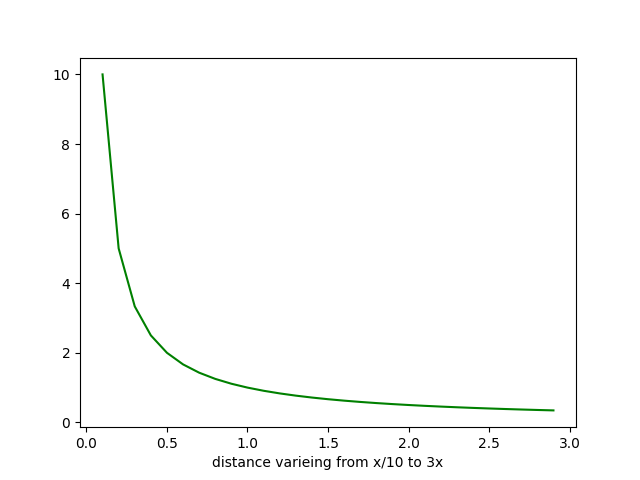
\includegraphics[width=.9\linewidth]{Pr2_plot.png}
\end{center}

In the current situation, the rate is \(5\times 10^{-2} Hz\) for the hit type T0. It will be varie from 0.5 to \(15\times 10^{-2}\).

\item[{(ii)}] In the current situation, L0 should happen in 10ns for L1. If we make it 20ns, the chance to happen L1 will be doubled. That also may reflect in the event rate. So, I think, the event rate will increase if we double the time window.
\end{description}

\section*{Question 4}
\label{sec:org39857dd}

\begin{description}
\item[{(a)}] The temperature of CMB is 2.725K. The, we can find the peak wavelength using Wein's displacement law. Then,

$$\lambda = \frac{b}{T} = \frac{2.898\times 10^{-3}}{2.725} = 1.06348\times 10^{-3} = 1.06348 mm$$
\end{description}
The Compton wavelength of proton is, \(\frac{h}{mc} = 1.32255489022\times 10^{-15}\)

Herem we can see that the compton wavelength of proton is much smaller than wavelength of photon. So, the scattering that happens in this case is Thomson scattering.But Thomson scattering occurs in the case of non-relativistic particle\footnote{Ref: \url{https://en.wikipedia.org/wiki/Thomson\_scattering}}. But, in the frame of proton before scattering, the proton will be non-relativistic. Then, the photon will be blue shifted.

The speed of this proton is 0.9999999999999999999999951c.

So, by applying the equation of blue shift,

$$\lambda_{obs} = \lambda \sqrt{\frac{1-\frac{v}{c}}{1+\frac{v}{c}}} = 1.72705904\times 10^{-15}$$
This also less than the compton wavelength of proton. So, let us upply Thomson scattering.

Then, the scattering cross section is,

$$\sigma_t = \frac{8\pi}{3}\left(\frac{\alpha \lambda_c}{2\pi}\right)^2 = 1.97762781004\times 10^{-35} m^2$$

Number density of CMB photons are around 411/cm\textsuperscript{3} or \(411\times 10^6 m^{-1}\).\footnote{Ref: \url{https://en.wikipedia.org/wiki/Cosmic\_microwave\_background}}

Then, the mean free path,

$$l = \frac{1}{n\sigma} = 1.23032 \times 10^{26} m$$

\begin{description}
\item[{(b)}] Diameter of milky way galaxy is around 10\textsuperscript{21}m. Distance to Andromeda Galaxy from earth is around 10\textsuperscript{22} m. But the mean free path of the ray is larger than this. That means it can come from a distance beyond this. That means, it may comeing from other galaxies. But, Greisen–Zatsepin–Kuzmin limit says, protons of energy higher than \(5\times 10^{19} eV\) cannot travel from other galaxies to earth. This is because of collision with CMB photons. But this says about the protons which travels between galaxies. But we had seen that the mean free path of the high energy photons is larger than Andromeda galaxy. So, if the parotons travelled a distance in that range only, it is possible to reach Earth. In that sense, this result is believable. But other thing is, GZK limit is not applicable for the cosmic rays made up of heavier elements. So, that is also a possibility in this case. In that sense also, this measurement is believable.\footnote{Ref: \url{https://en.wikipedia.org/wiki/Greisen\%E2\%80\%93Zatsepin\%E2\%80\%93Kuzmin\_limit}}

So, my conclusion is, it can be protons, which are produced in some process within a distance \(\sim 10^{26}m\). Since the mean free path is larger than this, it can reach earth. Or, it can be heavier elements, which GZK limit is not applicable.\footnote{Thanks to Akash Maurya for help.}
\end{description}

\section*{References}
\label{sec:org8254fdb}
\bibliography{../../../References/Bibliography}
\bibliographystyle{unsrt}
\end{document}